\documentclass{article}

\usepackage[utf8]{inputenc}
\usepackage{graphicx}
\usepackage{tikz}
\usepackage{float}
\usepackage{wrapfig,lipsum}
\usepackage{svg}
\usepackage{mathtools}
\usepackage{tabu}
\usepackage{subcaption}
\usepackage[a4paper, total={6in, 8in}]{geometry}


\begin{document}


\newcommand{\vecthreeBF}[1]{\vec{\textbf{#1}}}
\newcommand{\vecthree}[1]{\vec{#1}}

\newcommand{\parDeriv}[2]{\frac{\partial #1}{\partial #2}}
\newcommand{\parDerivS}[2]{\frac{\partial^2 #1}{\partial #2^2}}
\newcommand{\derivS}[2]{\frac{d^2 #1}{d#2^2}}

\newcommand{\dotProdBF}[2]{\vecthreeBF{#1} \cdot \vecthreeBF{#2}}
\newcommand{\dotProd}[2]{\vecthree{#1} \cdot \vecthree{#2}}

\newcommand{\crossProdBF}[2]{\vecthreeBF{#1} \times \vecthreeBF{#2}}
\newcommand{\crossProd}[2]{\vecthree{#1} \times \vecthree{#2}}


\newcommand{\fromeq}[1]{\textit{equation \ref{eq:#1}}}
\newcommand{\fromeqs}[2]{\textit{equations \ref{eq:#1} and \ref{eq:#2}}}

\newcommand{\fromfig}[1]{\textit{figure \ref{fig:#1}}}
\newcommand{\fromfigs}[2]{\textit{figures \ref{fig:#1} and \ref{fig:#2}}}
\newcommand{\fromsec}[1]{\textit{section \ref{sec:#1}}}

%----../../..++++.

%%%%%%

\section{Cavity Design} \label{sec:cavity_design}

The first and the most important design parameter for a cavity is the operating RF frequency.
After an operating RF frequency is set and the desired $R1/R2$ relation in \fromfig{pottier_table1} is selected, design parameters of acceleration plane of the cavity is fully determined.

By following the cylinderical design mentioned in \fromsec{theory_rhodo}, the only main design parameter remaining is the height of the cylindrical cavity.
This parameter can be found using the constraint mentioned in \fromsec{theory_cavities}; the fact that operating RF frequency must be equal to resonant frequency of the cavity.
For simple coaxial cavity, the height should be $\lambda/2$, where $\lambda$ is the wavelength of the external RF supply \cite{rhodo_pottier}.
Simulation tools such as \textit{CST Studio}, \textit{Poisson SUPERFISH} can be used to confirm this condition.

In the following examples, $p=1$ from \fromfig{pottier_table1} was used, and it will be the focus of all further calculations.
Using $f_{RF}=107.5$ MHz \& $f_{RF}=180$ MHz for comparison:
\begin{eqnarray} \label{eq:107_180_MHZ_cavity_design_parameters}
    \begin{aligned}
        f_{107.5} = 107.5 \textrm{ MHz} \\
        \lambda_{107.5}  = \frac{c}{f_{107.5}} = 2.789 m \\
        R_2 = 0.27 \times \lambda_{107.5} = 0.753 m \\
        R_1 = \frac{R_2}{4} = 0.188 m \\
        h = \frac{\lambda}{2} = 1.394 m 
    \end{aligned}
    \qquad\qquad
    \begin{aligned}
        f_{180} = 180 \textrm{ MHz} \\
        \lambda_{180}  = \frac{c}{f_{180}} = 1.666 m \\
        R_2 = 0.27 \times\lambda_{180} = 0.450 m \\
        R_1 = \frac{R_2}{4} = 0.113 m \\
        h = \frac{\lambda}{2} = 0.833 m 
    \end{aligned}
\end{eqnarray}
In the following figures, \textit{Poisson Superfish} and \textit{CST} simulations of two cavities defined by \fromeq{107_180_MHZ_cavity_design_parameters} can be observed.
\begin{figure}[H]
    \centering
    \begin{subfigure}{.5\textwidth}
      \centering
      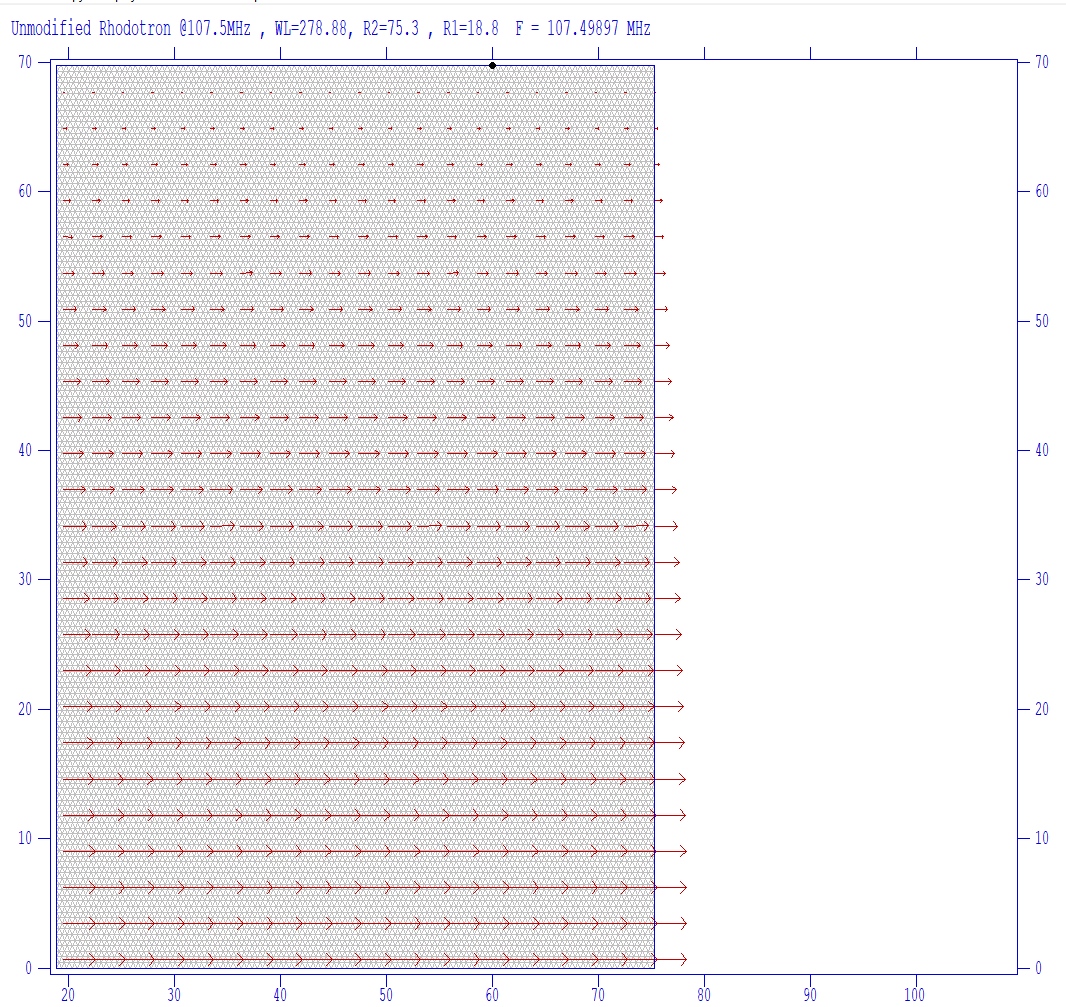
\includegraphics[width=\linewidth]{../../../figures/superfish/superfish107.png}
      \caption{107.5 MHz}
    \end{subfigure}%
    \centering
    \begin{subfigure}{.5\textwidth}
      \centering
      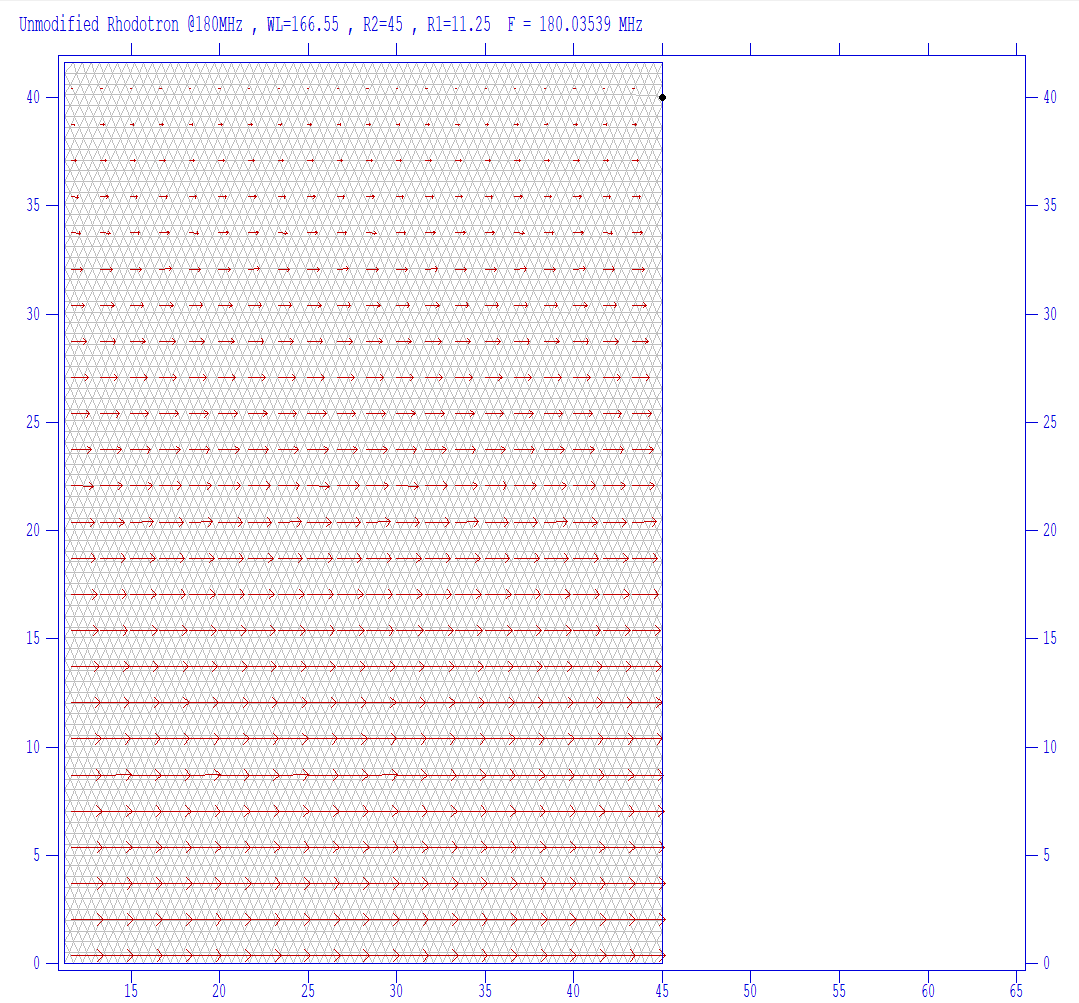
\includegraphics[width=\linewidth]{../../../figures/superfish/superfish180.png}
      \caption{180 MHz}
    \end{subfigure}
    \caption{Poission Superfish results for \fromeq{107_180_MHZ_cavity_design_parameters}}
    \label{fig:107_simple_cavity_design}
\end{figure}

\begin{figure}[H]
    \centering
    \begin{subfigure}{.5\textwidth}
      \centering
      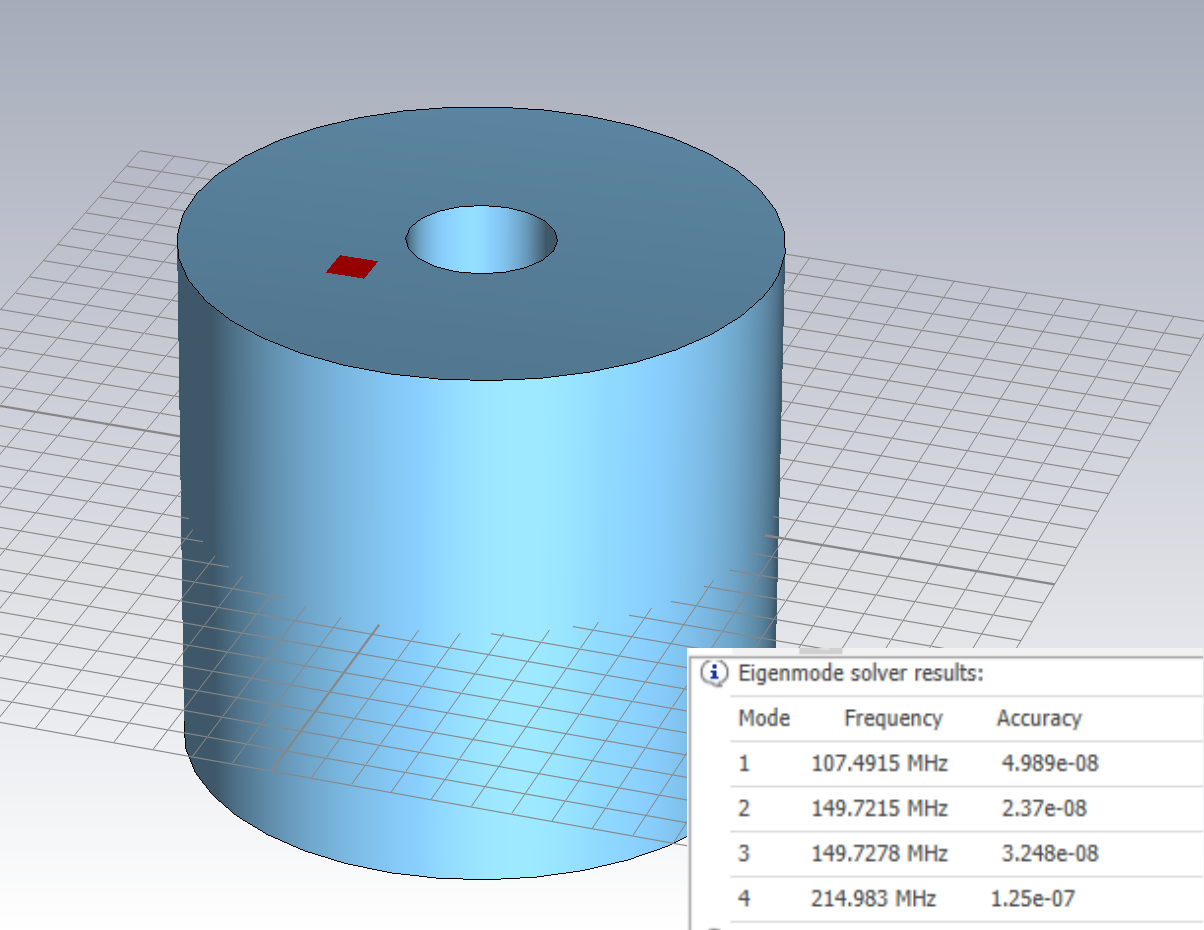
\includegraphics[width=\linewidth]{../../../figures/cst/cst107.png}
      \caption{107.5 MHz}
    \end{subfigure}%
    \begin{subfigure}{.5\textwidth}
      \centering
      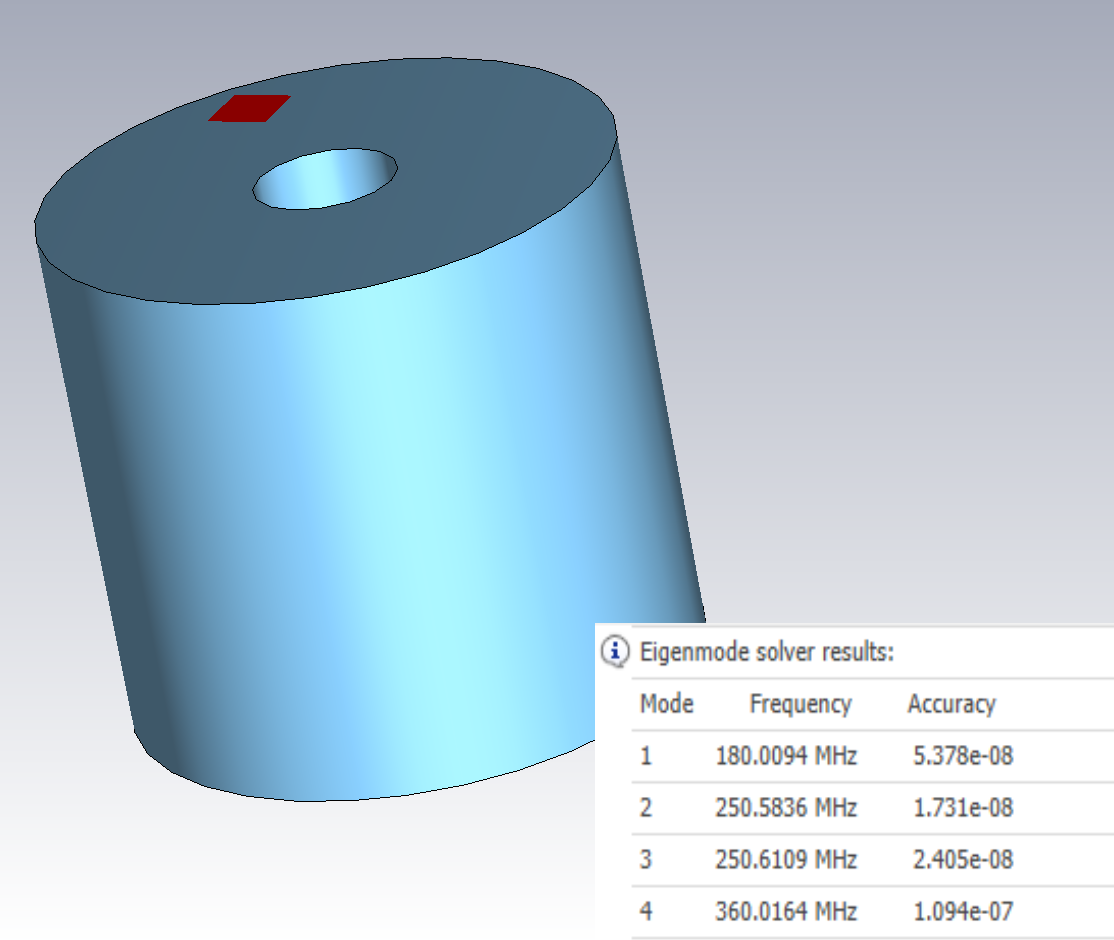
\includegraphics[width=.9\linewidth]{../../../figures/cst/cst180.png}
      \caption{180 MHz}
    \end{subfigure}
    \caption{CST Eigenmode results for \fromeq{107_180_MHZ_cavity_design_parameters}}
    \label{fig:180_simple_cavity_design}
\end{figure}

\begin{figure}[H]
    \centering
    \begin{subfigure}{.5\textwidth}
      \centering
      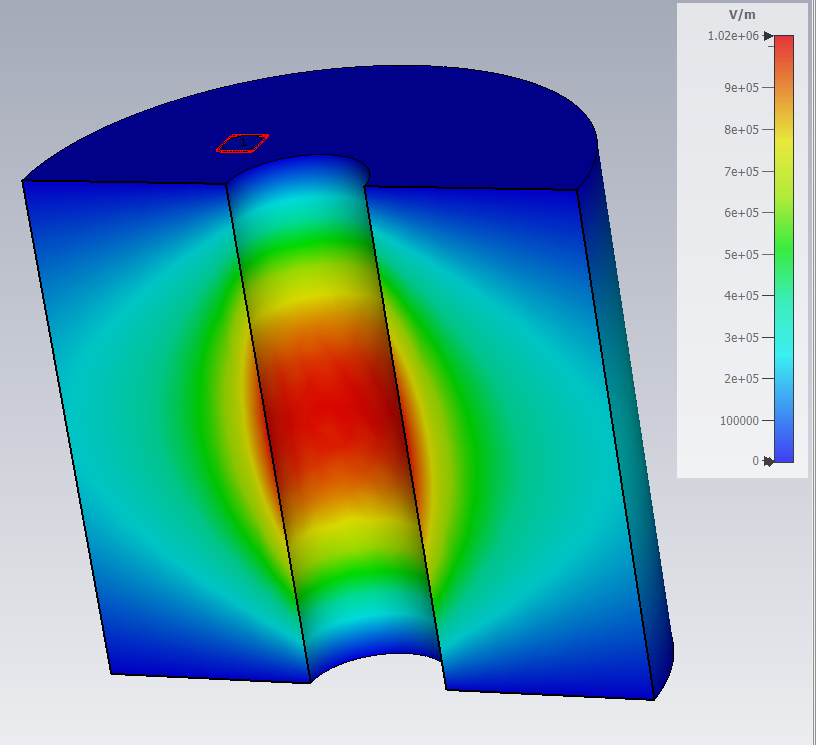
\includegraphics[width=.9\linewidth]{../../../figures/cst/cst107_e.png}
      \caption{107.5 MHz}
    \end{subfigure}%
    \begin{subfigure}{.5\textwidth}
      \centering
      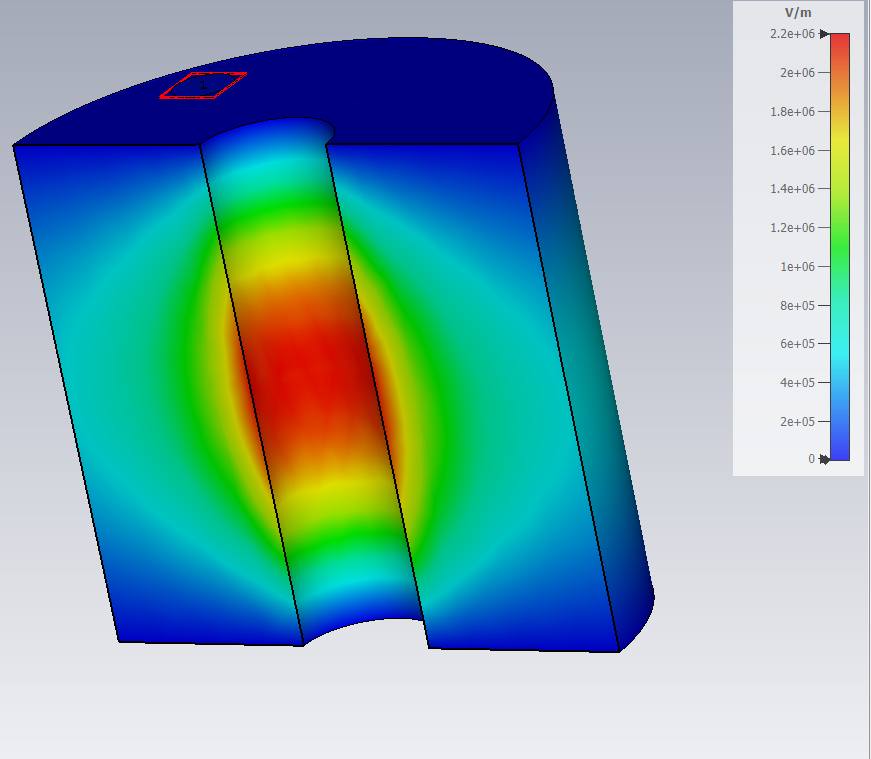
\includegraphics[width=.94\linewidth]{../../../figures/cst/cst180_e.png}
      \caption{180 MHz}
    \end{subfigure}
    \caption{CST Electric field solutions for \fromeq{107_180_MHZ_cavity_design_parameters}}
    \label{fig:cst_simple_cavity_designs}
\end{figure}
As mentioned by POTTIER, truncated cone terminations in inner cylinder can improve the shunt empedance $Z$ of the cavity \cite{rhodo_pottier}. 
Below, \textit{Poission superfish} results of such a modification with matching height increase to keep resonant frequency can be found.
\begin{figure}[H]
    \centering
    \begin{subfigure}{.5\textwidth}
      \centering
      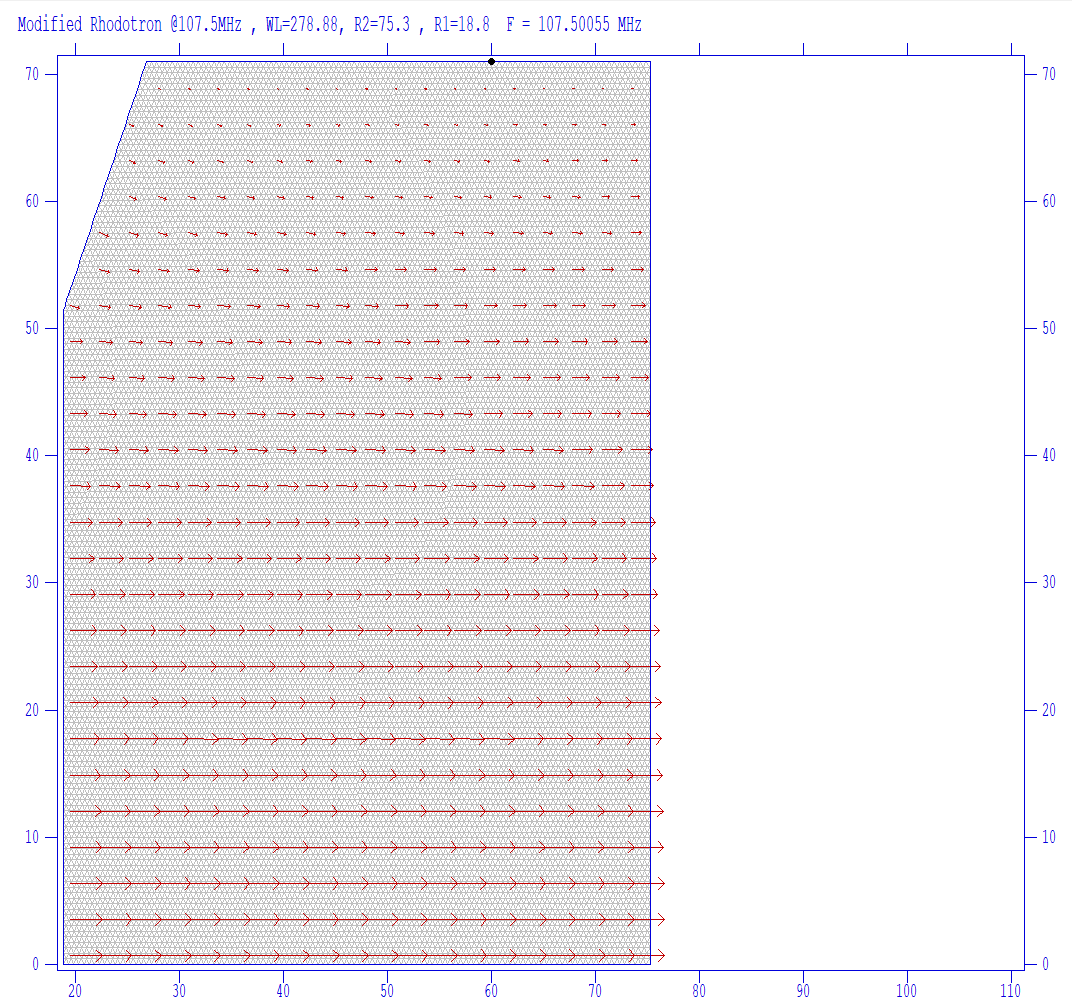
\includegraphics[width=.9\linewidth]{../../../figures/superfish/superfish107mod.png}
      \caption{107.5 MHz truncated}
    \end{subfigure}%
    \begin{subfigure}{.5\textwidth}
      \centering
      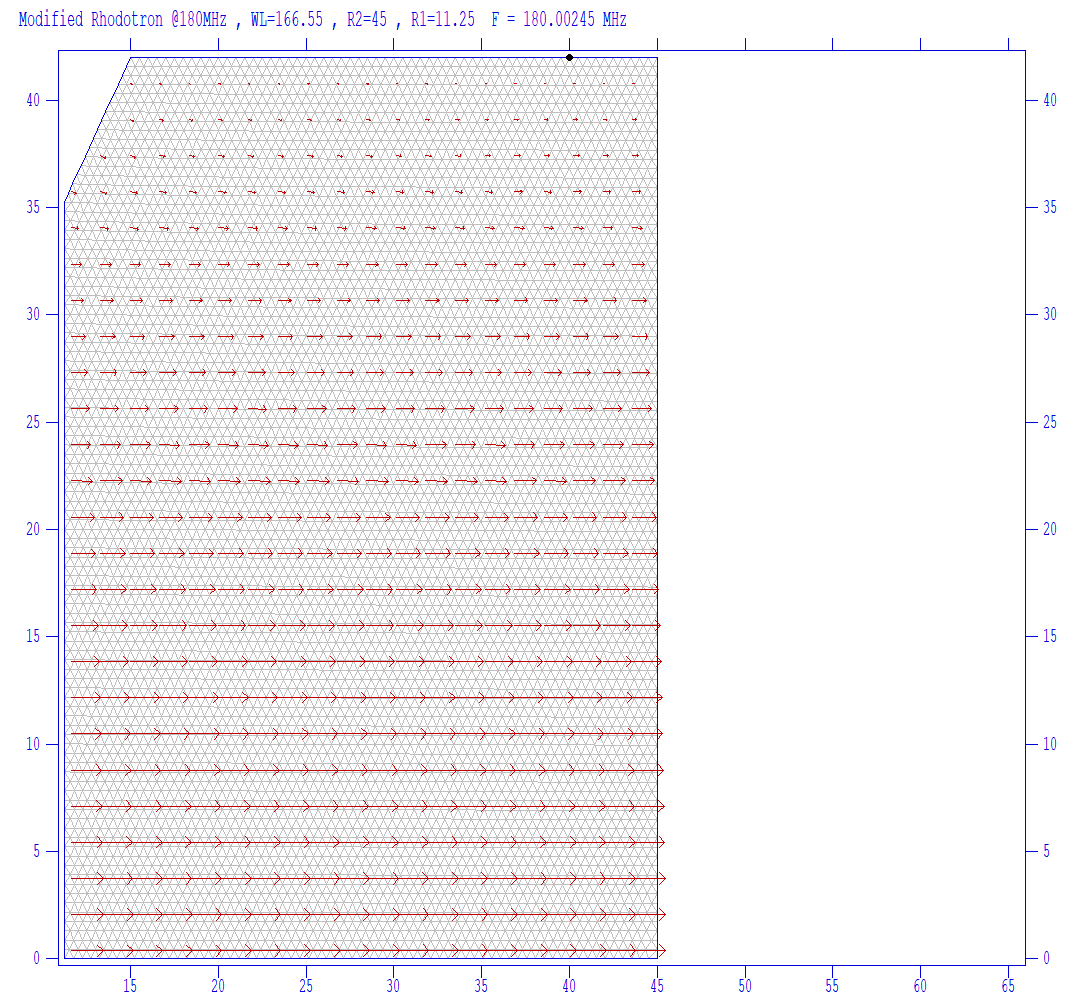
\includegraphics[width=.9\linewidth]{../../../figures/superfish/superfish180mod.png}
      \caption{180 MHz truncated}
    \end{subfigure}
    \caption{Poisson SUPERFISH field results of truncated cavities}
    \label{fig:107_180_modified_cavities_superfish}
\end{figure}

\begin{figure}[H]
    \centering
    \begin{subfigure}{.5\textwidth}
      \centering
      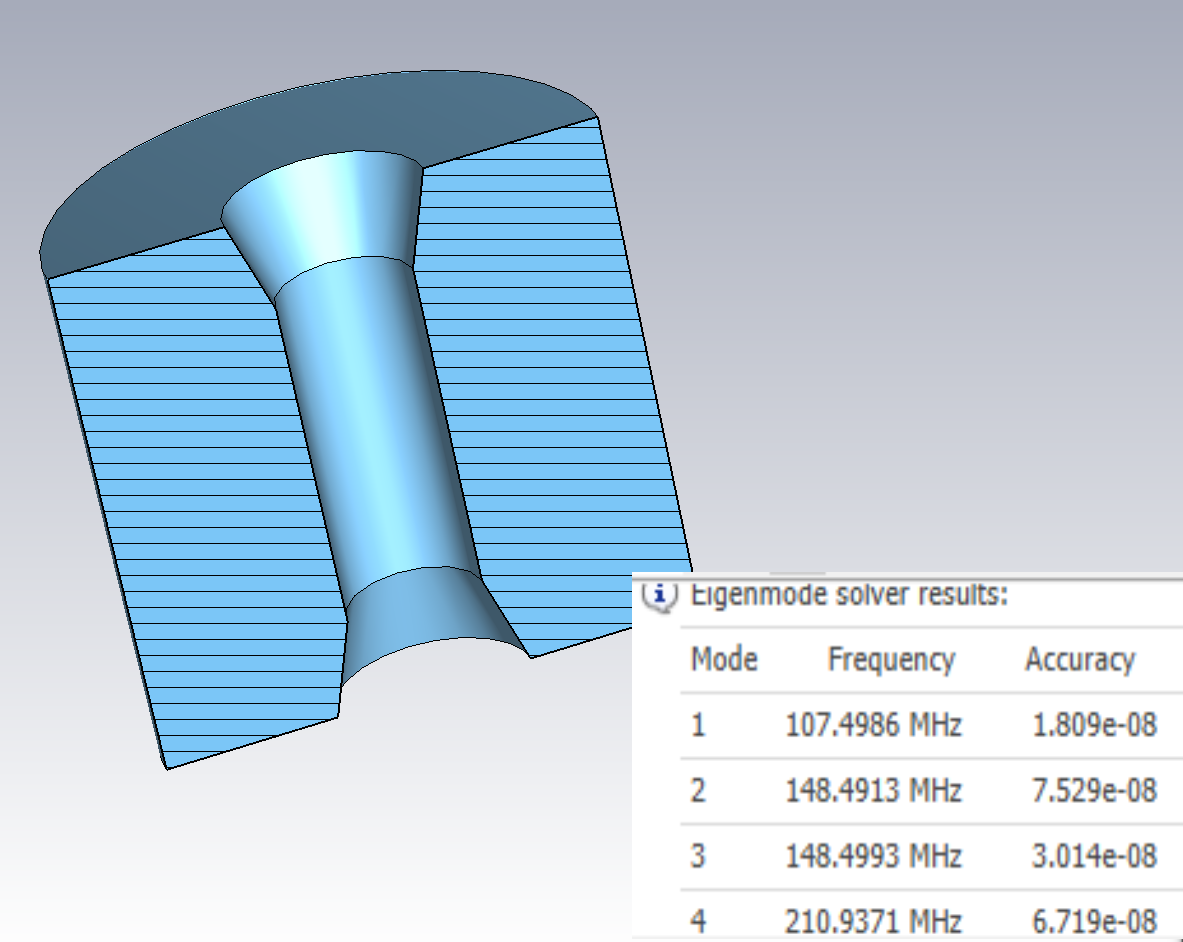
\includegraphics[width=.9\linewidth]{../../../figures/cst/cst107mod.png}
      \caption{107.5 MHz truncated}
    \end{subfigure}%
    \begin{subfigure}{.5\textwidth}
      \centering
      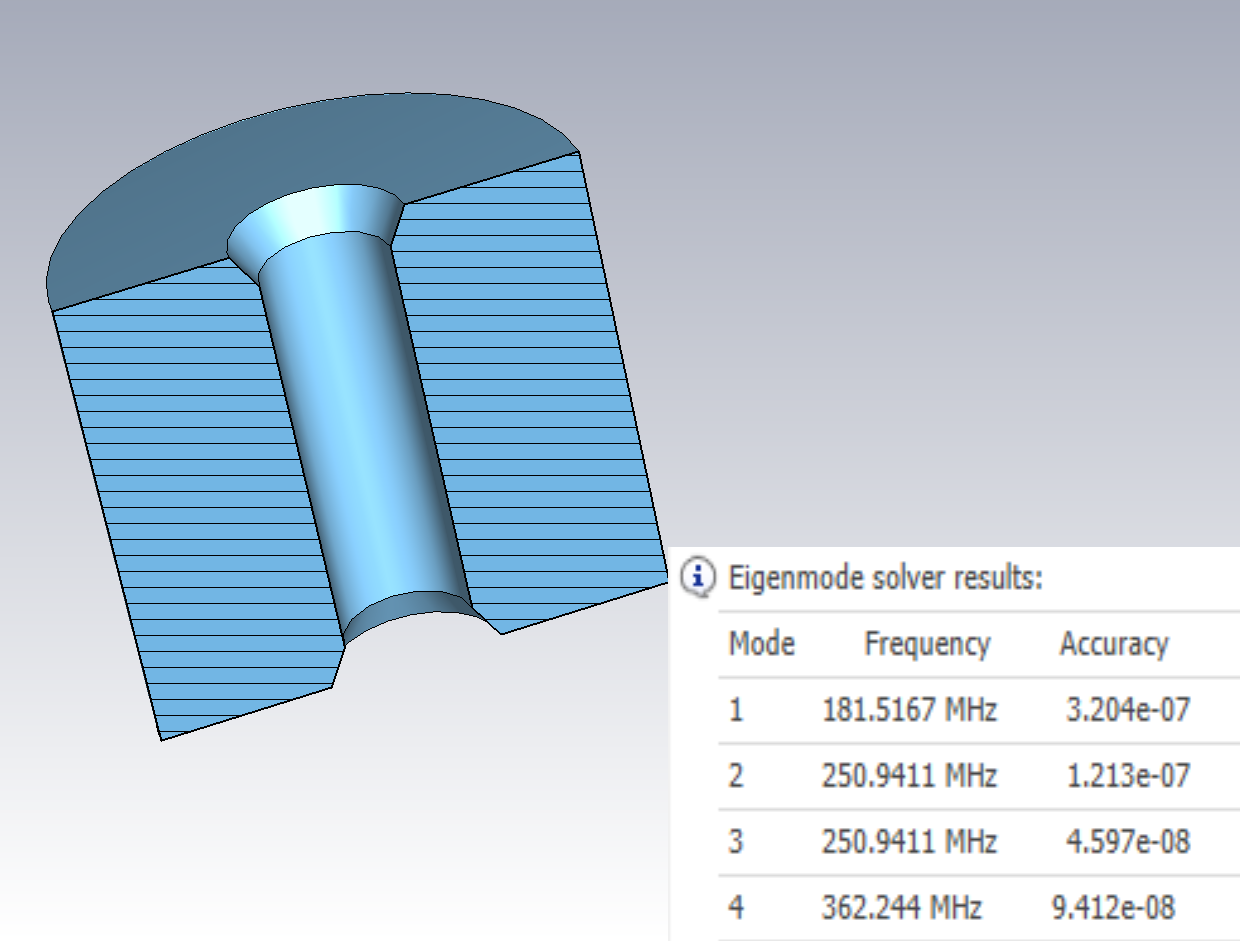
\includegraphics[width=.9\linewidth]{../../../figures/cst/cst180mod.png}
      \caption{180 MHz truncated}
    \end{subfigure}
    \caption{CST eigenmode results of truncated cavities}
    \label{fig:107_180_modified_cavities_cst_eigenmode}
\end{figure}

\begin{figure}[H]
    \centering
    \begin{subfigure}{.5\textwidth}
      \centering
      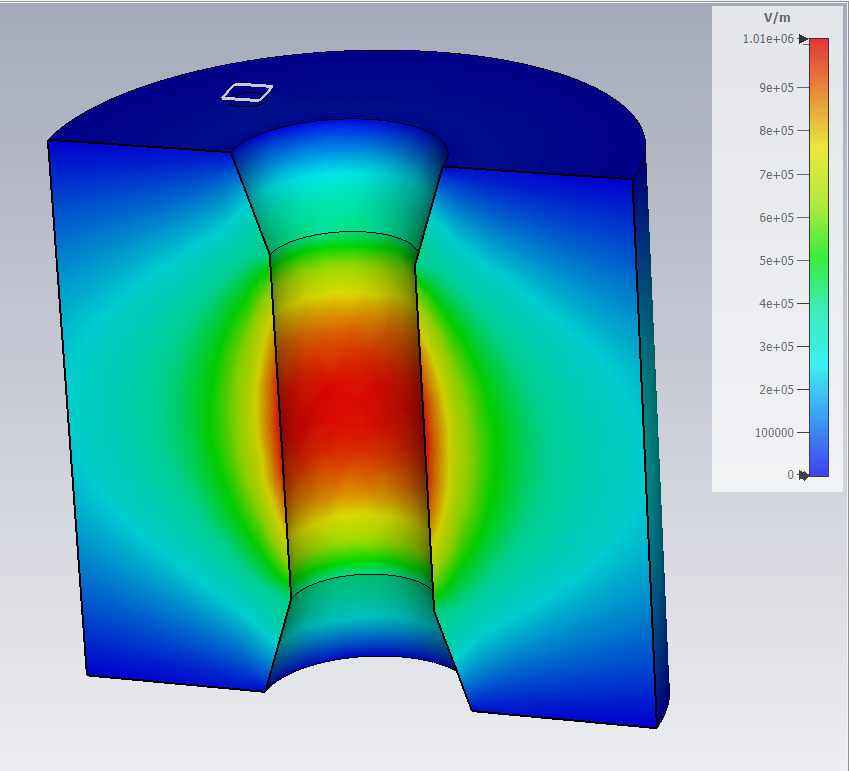
\includegraphics[width=.9\linewidth]{../../../figures/cst/cst107mod_e.png}
      \caption{107.5 MHz truncated}
    \end{subfigure}%
    \begin{subfigure}{.5\textwidth}
      \centering
      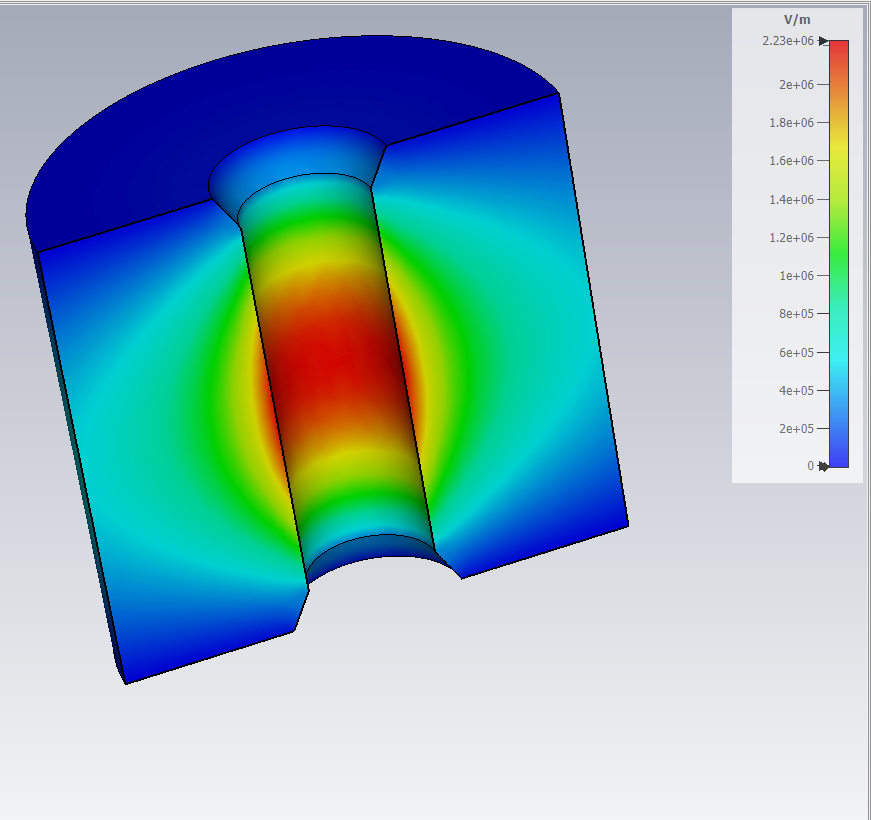
\includegraphics[width=.88\linewidth]{../../../figures/cst/cst180mod_e.png}
      \caption{180 MHz truncated}
    \end{subfigure}
    \caption{CST electric field results of truncated cavities}
    \label{fig:107_180_modified_cavities_cst_field}
\end{figure}

\begin{figure}[H]
    \centering
    \begin{subfigure}{.5\textwidth}
      \centering
      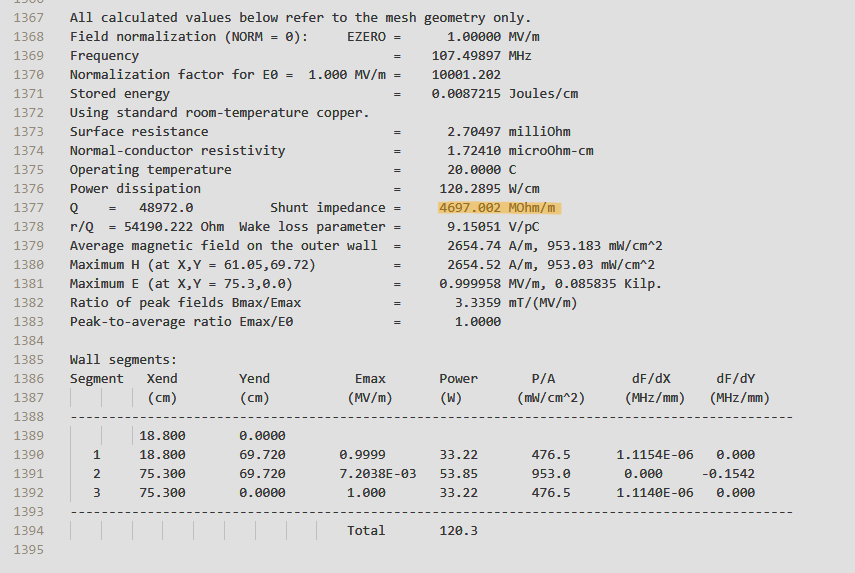
\includegraphics[width=0.97\linewidth]{../../../figures/superfish/superfish107_z_highlighted.png}
      \caption{107.5 MHz unmodified}
    \end{subfigure}%
    \begin{subfigure}{.5\textwidth}
      \centering
      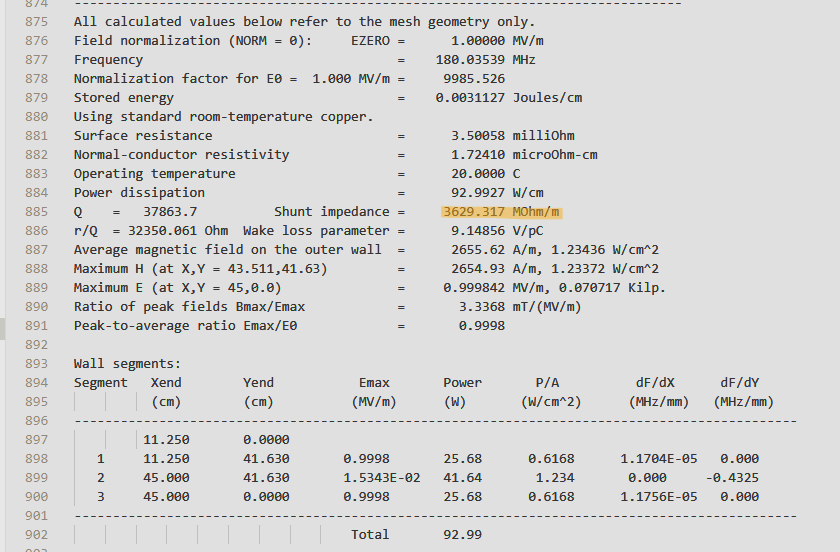
\includegraphics[width=0.99\linewidth]{../../../figures/superfish/superfish180_z_highlighted.png}
      \caption{180 MHz unmodified}
    \end{subfigure}
    \caption{Poisson Superfish calculations with \textit{unmodified} cavities}
    \label{fig:107_cavity_shunt_diff}
\end{figure}
    
\begin{figure}[H]
    \centering
    \begin{subfigure}{.5\textwidth}
      \centering
      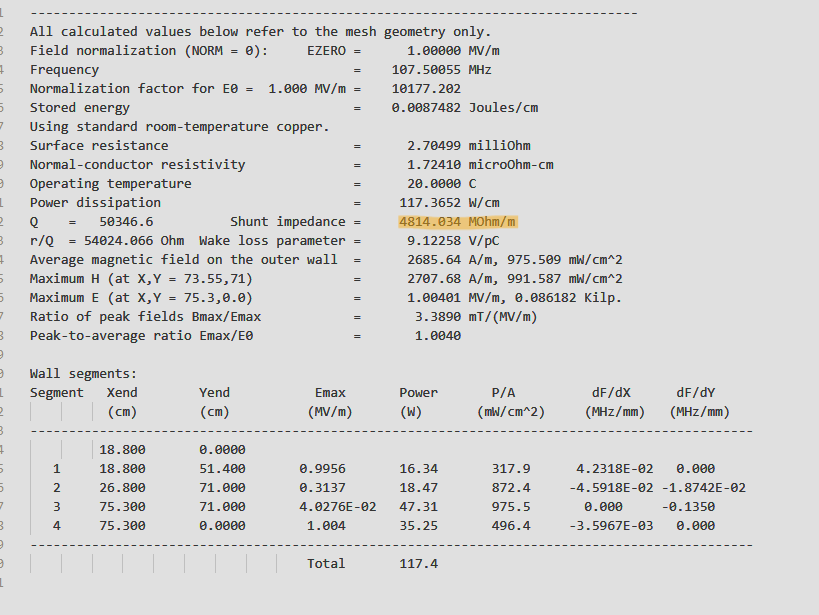
\includegraphics[width=0.95\linewidth]{../../../figures/superfish/superfish107mod_z_highlighted.png}
      \caption{107.5 MHz truncated}
    \end{subfigure}%
    \begin{subfigure}{.5\textwidth}
      \centering
      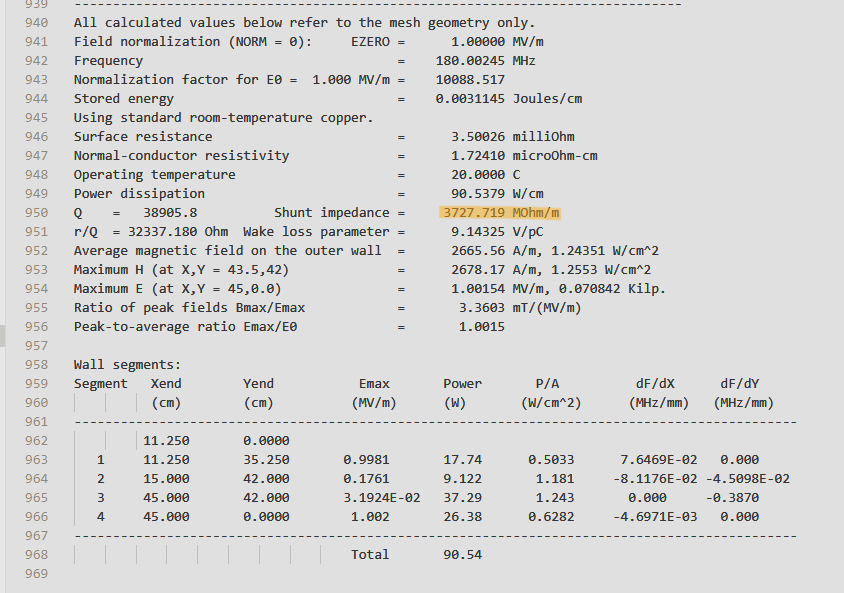
\includegraphics[width=\linewidth]{../../../figures/superfish/superfish180mod_z_highlighted.png}
      \caption{180 MHz truncated}
    \end{subfigure}
    \caption{Poisson Superfish calculations with \textit{truncated} cavities}
    \label{fig:180_cavity_shunt_diff}
\end{figure}
One can observe the shunt impedance gain between truncated and unmodified cavities in \fromfigs{107_cavity_shunt_diff}{180_cavity_shunt_diff};
\begin{equation*}
    \begin{aligned}
        \Delta Z_{107.5}=2.5\%
    \end{aligned}
    \qquad
    \begin{aligned}
        \Delta Z_{180}=2.7\%
    \end{aligned}
\end{equation*}

%%%%%%


\end{document}